% $Id: board1.tex 9716 2021-12-18 23:18:03Z mskala $

%
% MSK 009 Board 1 build instructions
% Copyright (C) 2018, 2020, 2021  Matthew Skala
%
% This program is free software: you can redistribute it and/or modify
% it under the terms of the GNU General Public License as published by
% the Free Software Foundation, version 3.
%
% This program is distributed in the hope that it will be useful,
% but WITHOUT ANY WARRANTY; without even the implied warranty of
% MERCHANTABILITY or FITNESS FOR A PARTICULAR PURPOSE.  See the
% GNU General Public License for more details.
%
% You should have received a copy of the GNU General Public License
% along with this program.  If not, see <http://www.gnu.org/licenses/>.
%
% Matthew Skala
% https://northcoastsynthesis.com/
% mskala@northcoastsynthesis.com
%


\chapter{Building Board 1}\label{ch:board1}

Board~1 has components on both sides, and for best results, it is important
to install them in the right order.  Build Board~2 first, and see the
general comments in the Board~2 chapter about how to approach the task.

\section{Preliminaries}

Count out the right number of everything according to the bill of materials. 
There is an abbreviated BOM for the items needed in this chapter (including
the connection to Board~2 and final assembly of the module) in
Table~\ref{tab:b1bom}.

\nopagebreak
\noindent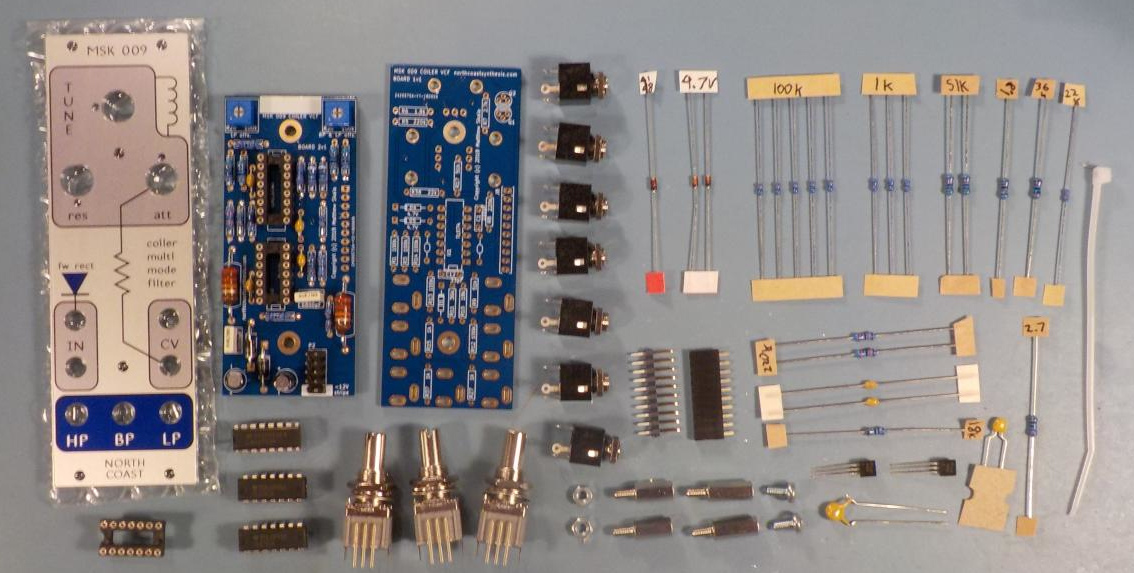
\includegraphics[width=\linewidth]{board1-parts.jpg}

\begin{table*}
{\centering
\fbox{This table is not a substitute for the text instructions.}
\vspace{\baselineskip}

\begin{tabular}{rp{1.3in}cp{3in}}
  \textbf{Qty} & \textbf{Ref} & \textbf{Value/Part No.} & \\ \hline
\input{bomdata-1.tex}
\end{tabular}\par}
\caption{Bill of Materials for Board~1.  Newer kits may include TL074B
op amps instead of TL074, to make offset nulling easier.  Also needed:
the PCB itself, the aluminum front panel, knobs, a cable tie,
the assembled Board~2, and panel-to-rack mounting hardware.}\label{tab:b1bom}
\end{table*}

\section{Some notes on knobs}

The first batch of knobs I ordered for North Coast products turned out to
have serious quality problems, specifically with the setscrews that hold the
knobs onto the potentiometer shafts.  Some of the screws had marginal
threads that would strip when the screw was tightened, and I ended up having
to do a bunch of extra testing and ship extra knobs to some customers to
replace any that might fail.  Later batches have also had issues, although
they're under better control now because the bad first batch served as a
warning to step up the testing procedures.  Starting with kits prepared in
August 2019, I switched to blue knobs with 100\%\ testing; in September
2020, I switched to a new manufacturer, and knobs that are a slightly darker
shade of blue.  Although all the knobs I ship in kits now have been tested
and passed at least twice, and should be fine to use, I am also shipping
spare setscrews in any kits with knobs from batches where a signficant
number of knobs failed testing.

Here are some things to be aware of as a kit builder.

\begin{itemize}
\item Some photos in these instructions were taken with the older grey
knobs, and some dealers will still have kits containing grey knobs in their
stock, but newer kits will have blue knobs.

\item Do not overtighten the setscrews when attaching the knobs!  The screw
should be tight enough to hold the knob onto the shaft, but there's no
advantage to making it tighter than that, and overtightening may risk
destroying the screw thread or damaging the drive slot.

\item If, despite my efforts to make sure no bad screws get sent to
customers, you still get a bad screw that cannot be tightened and no spare
for it, then please contact me.

\item If you want to source an exact replacement for the setscrew, it should
be an M3$\times$3mm flat-tip slotted setscrew, which is also sometimes
called a ``grub screw,'' made of RoHS-compliant brass (possibly by
exemption).  Stainless steel is fine too, and I may sometimes ship stainless
steel screws instead of brass if I can find a reliable source for them;
plain steel should not be used here for galvanic corrosion reasons. 
Hex-socket screws are fine if you have the driver for them, but I don't ship
those because I'm not sure all DIY builders do have the right driver.

\item Because it's a standard M3 thread, in a pinch it's possible to
substitute a plain M3 machine screw such as are commonly used with Eurorack
cases, although one of those would obviously look less nice.
\end{itemize}

\pagebreak

\section{Decoupling capacitors}

The two axial ceramic 0.1$\mu$F decoupling capacitors C6 and C7 are shown on
the board by a special symbol without their reference designators.

\nopagebreak
\noindent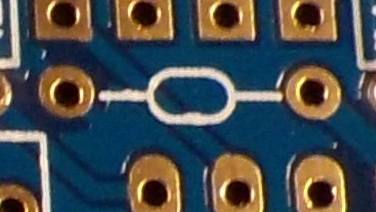
\includegraphics[width=\linewidth]{decoup-symbol.jpg}

Install these two capacitors where the symbol appears.  They are not
polarized and may be installed in either orientation.  These capacitors act
as filters for the power supplies to the op amp chip, protecting them from
high-frequency crosstalk.

\nopagebreak
\noindent\includegraphics[width=\linewidth]{{cap-0.1u1}.jpg}

\section{Fixed resistors}

Resistors are never polarized.  I like to install mine in a consistent
direction for cosmetic reasons, but this is electrically unnecessary.  In
this module, the fixed resistors are metal film 1\%\ type.  They usually
have blue bodies and four colour bands designating the value, plus a fifth
band for the tolerance.  The tolerance band is brown for 1\%, but note that
we may occasionally ship better-tolerance resistors in the kits than the
specifications require, if we are able to source them at a good price. 
Accordingly, I mention only the four value band colours for this type of
resistor; if you are using resistors with other codes, you are responsible
for knowing them.  Note that colour codes on metal film 1\% resistors are
often ambiguous (reading from one end or the other end may give two
different values, both plausible) and some of the colours are hard to
distinguish anyway.  If in doubt, always measure with an ohmmeter before
soldering the resistor in place.

Install the three 1k$\Omega$ (brown-black-black-brown) resistors R15, R27,
and R37.  These are current-limiting resistors to protect the audio outputs,
and other modules, in case of short circuits or bad patching.

\nopagebreak
\noindent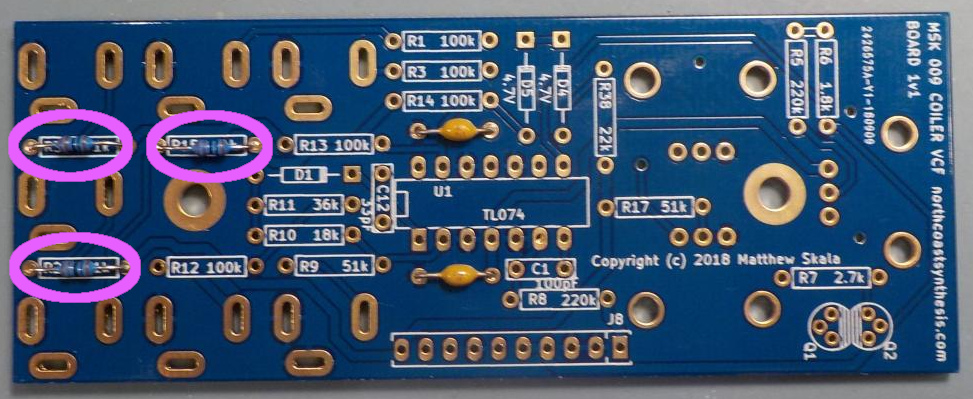
\includegraphics[width=\linewidth]{res-1k.jpg}

Install the 1.8k$\Omega$ (brown-grey-black-brown) resistor R6.  This is the
feedback resistor for the CV-processing op amp, setting the CV sensitivity
to approximately 1V/octave.  Do not confuse this with the 18k$\Omega$
resistor, which has a similar colour code.

\nopagebreak
\noindent\includegraphics[width=\linewidth]{{res-1.8k}.jpg}

Install the 2.7k$\Omega$ (red-violet-black-brown) resistor R7.  This is a
ballast resistor for the temperature-servo op amp, preventing the voltage
gain of the transistor in the feedback loop from rendering the amplifier
unstable.

\nopagebreak
\noindent\includegraphics[width=\linewidth]{{res-2.7k}.jpg}

Install the 18k$\Omega$ (brown-grey-black-red) resistor R10.  This resistor
is used to control the gain in the full-wave rectifier circuit.

\nopagebreak
\noindent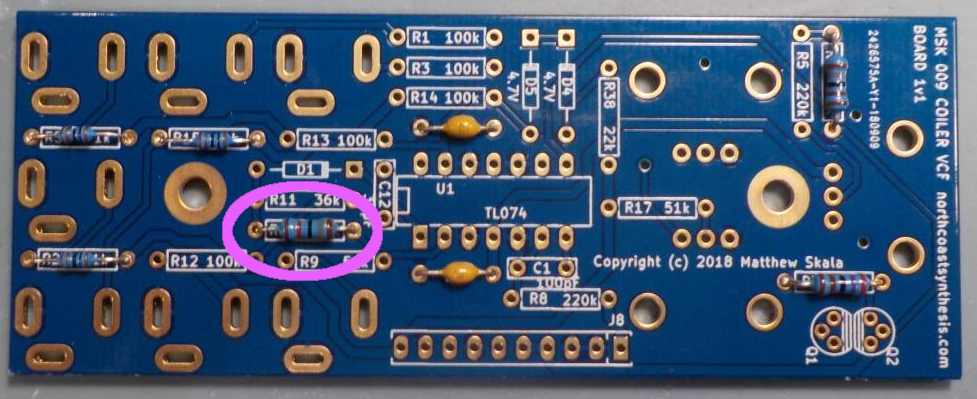
\includegraphics[width=\linewidth]{res-18k.jpg}

Install the 22k$\Omega$ (red-red-black-red) resistor R38.  This resistor
controls the amount of clipping applied on an internal feedback path,
to set the amplitude level during oscillation.  Do not confuse this resistor
with the 220k$\Omega$ resistors, which have a similar colour code.

\nopagebreak
\noindent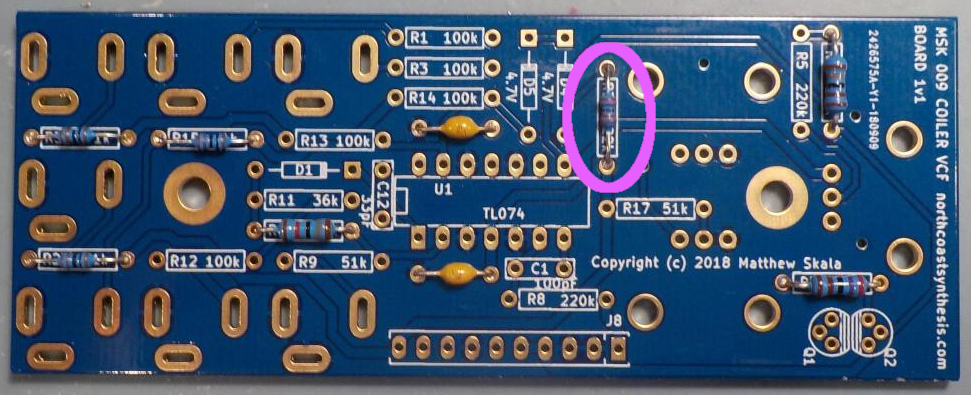
\includegraphics[width=\linewidth]{res-22k.jpg}

Install the 36k$\Omega$ (orange-blue-black-red) resistor R11.  This controls
the level of the full-wave rectified input signal applied to the input mixer.

\nopagebreak
\noindent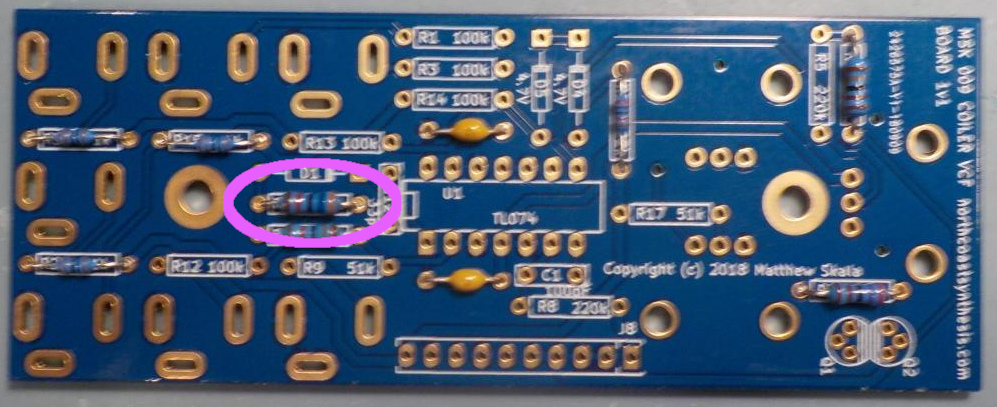
\includegraphics[width=\linewidth]{res-36k.jpg}

Install the two 51k$\Omega$ (green-brown-black-red) resistors R9 and R17. 
These are used for level and impedance control:  R9 on the rectifier input,
and R17 on the internal BP feedback path.

\nopagebreak
\noindent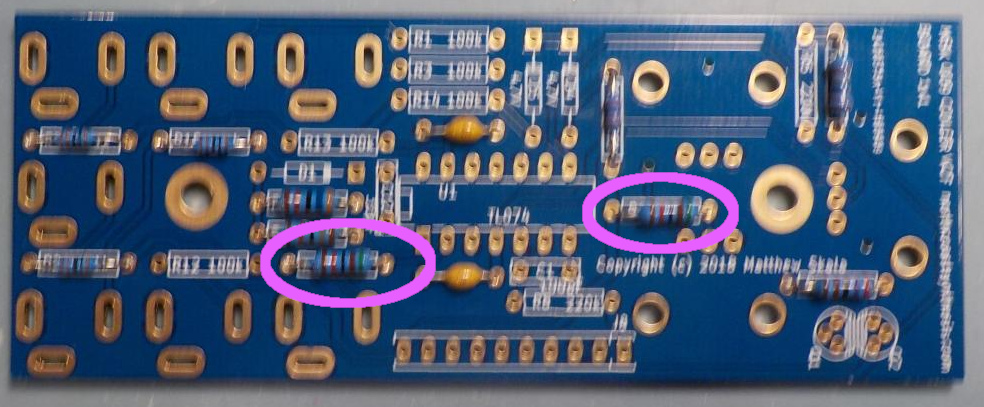
\includegraphics[width=\linewidth]{res-51k.jpg}

Install the five 100k$\Omega$ (brown-black-black-orange) resistors R1, R3,
R12, R13, and R14.  The first three of these are used to set input
impedances for the unrectified audio input and both CV inputs.  The
remaining two, R13 and R14, set gain levels in the input mixer.

\nopagebreak
\noindent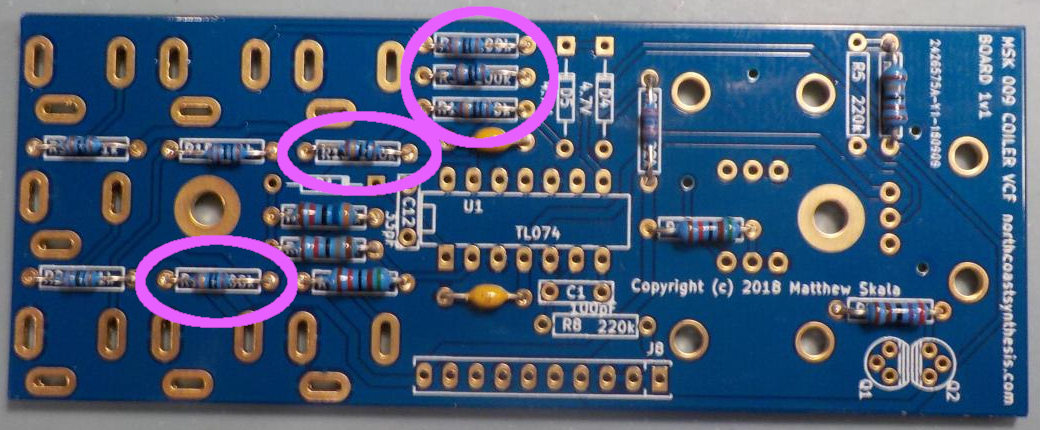
\includegraphics[width=\linewidth]{res-100k1.jpg}

\pagebreak

Install the two 220k$\Omega$ (red-red-black-orange) resistors R5 and R8. 
The first, R5, controls the scale of the main tuning knob; the
second, R8, contols the reference current for the exponential converter.

\nopagebreak
\noindent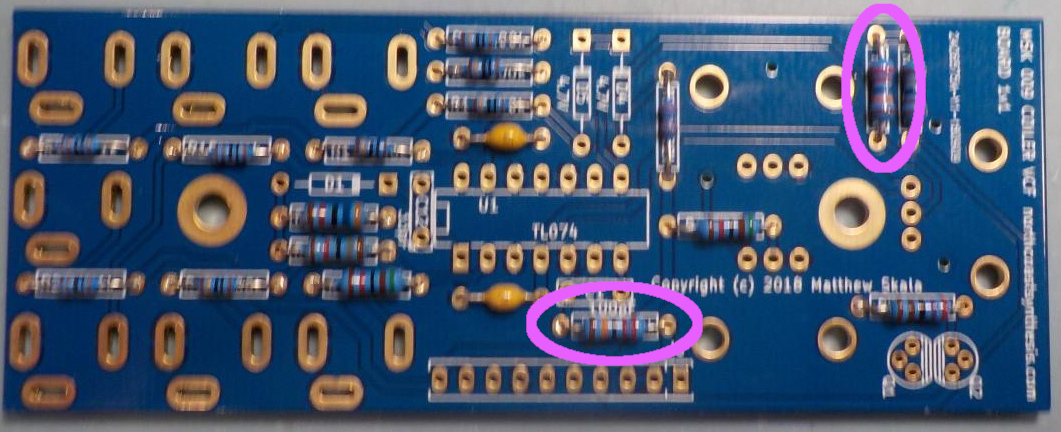
\includegraphics[width=\linewidth]{res-220k1.jpg}

\section{Semiconductors}

There are two different kinds of diodes to install on this board and they
look almost exactly alike: one 1N4148 or 1N914 switching diode named D1, and
two 1N5230B or equivalent 4.7V Zener diodes named D4 and D5.  All three
diodes will be packaged in little pink glass beads with near-microscopic
etched numbers indicating their type.  Be careful not to confuse them;
swapping the switching diode with a Zener will result in incorrect behaviour
of the full-wave rectifier at high input voltages, and incorrect feedback
levels probably causing either very strong oscillation at all resonance
settings, or preventing oscillation entirely.

If you are unsure which diode is which and you cannot confidently read the
etched markings, hook up a diode in series with a 10k$\Omega$ resistor
reverse-biased across a 12V power supply and measure the voltage drop across
the diode.  If it is near 12V, then you are testing the switching diode; if
it is near 4.7V, you are testing one of the Zener diodes; if it is near
0.6V, you probably have the diode connected forward-biased and should
reverse the polarity of it or the power supply.

Both kinds of diodes are polarized and must be installed in the correct
direction to function properly.  One end of the glass body of the diode
package will be labelled with a black band or stripe; that end is the
\emph{cathode}.  The direction for the cathode is marked on the PCB
silkscreen by a matching stripe in the printed symbol; and the solder pad
for the cathode is square rather than round.  The note ``4.7V'' is also
on the PCB silkscreen next to the locations of the two Zener diodes as
an added reminder of which diode goes where.

\pagebreak

Install the switching diode D1, bearing in mind the notes above.  This diode
is used in the full-wave rectifier to switch between inverting and
non-inverting modes.

\nopagebreak
\noindent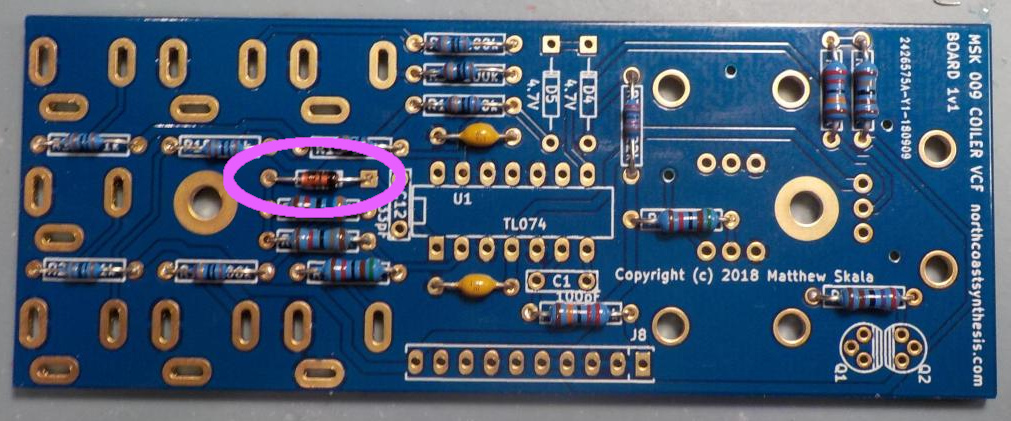
\includegraphics[width=\linewidth]{1n4148.jpg}

Install the two 4.7V Zener diodes D4 and D5.  These apply clipping to the BP
feedback path, setting the amplitude level during oscillation.

\nopagebreak
\noindent\includegraphics[width=\linewidth]{{zener-4.7v}.jpg}

Install the 14-pin DIP socket for the TL074 quad operational
amplifier (op amp) U1.  Two of the four amplifiers on this chip form the
exponential converter, which converts the tuning inputs into a control
current for the core.  One more is the full-wave rectifier for the rectified
input, and the last amplifier is part of the filter core, mixing the input
signals with the feedback paths to generate the HP signal.

DIP sockets
themselves do not care which direction you install them, but it is
critically important that the chip installed in the socket should be
installed in the right direction.  To help with that, the socket will
probably be marked with notches at one end (indicating the end where Pin~1
and Pin~14 are located) and you should install the socket so that the
notched end matches the notch shown on the PCB silkscreen.  The solder pad
for Pin~1 is also distinguished by being rectangular instead of rounded.

Installing DIP sockets without having them tilted at a funny angle can be
tricky.  I recommend inserting the socket in the board, taping it in place
on the component side with vinyl electrical tape or sticking it there with a
small blob of putty at each end, then soldering one pin on
one corner and checking that the socket is snug against the board before
soldering the other pins.  That way, if you accidentally solder the first
pin with the socket tilted, it will be easier to correct (only one pin to
desolder instead of all of them).

\nopagebreak
\noindent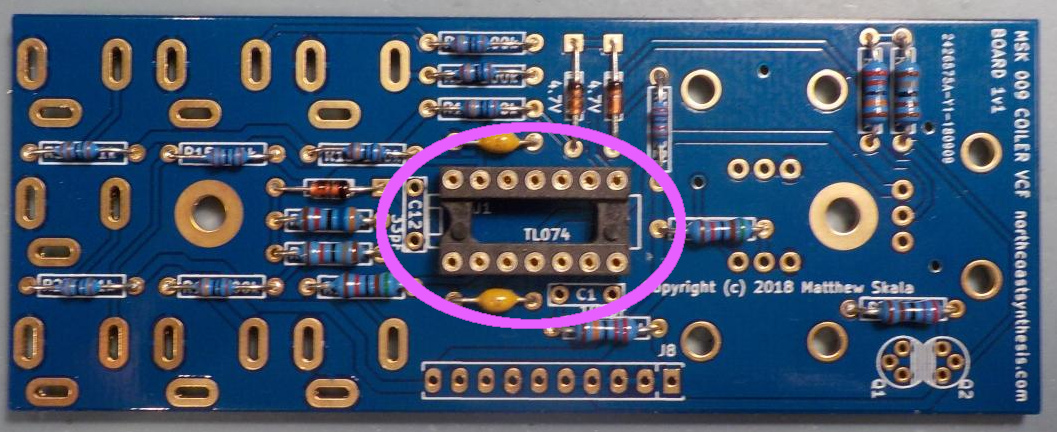
\includegraphics[width=\linewidth]{dip14-1.jpg}

\section{Compensation capacitors}

Install the 33pF radial ceramic capacitor C12.  It will probably be marked
``330,'' which means 33pF in a scheme similar to the resistor colour code:
significant digits 3 3 to be followed by 0 zeroes.  This capacitor helps
ensure stability of the input mixer op amp, and the filter core as a whole,
by killing the frequency response at frequencies above audio.  Without it,
the nonideal behaviour of the inductors could turn the filter core into a
low-frequency radio transmitter.  This capacitor is not polarized and may be
installed in either direction.

\nopagebreak
\noindent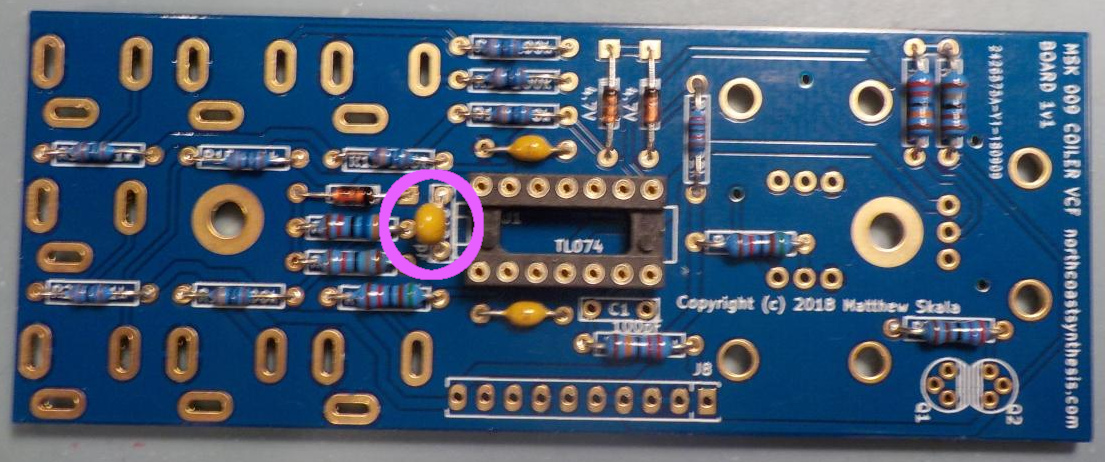
\includegraphics[width=\linewidth]{cap-33p.jpg}

Install the 100pF radial ceramic capacitor C1.  This similarly is a
stability enhancer for the servo op amp in the exponential converter,
preventing the amplifier from oscillating at high frequency.  The capacitor
will probably be marked ``101,'' for 1 0 followed by one more 0 number of
picofarads.  It is not polarized and may be installed in either direction.

\nopagebreak
\noindent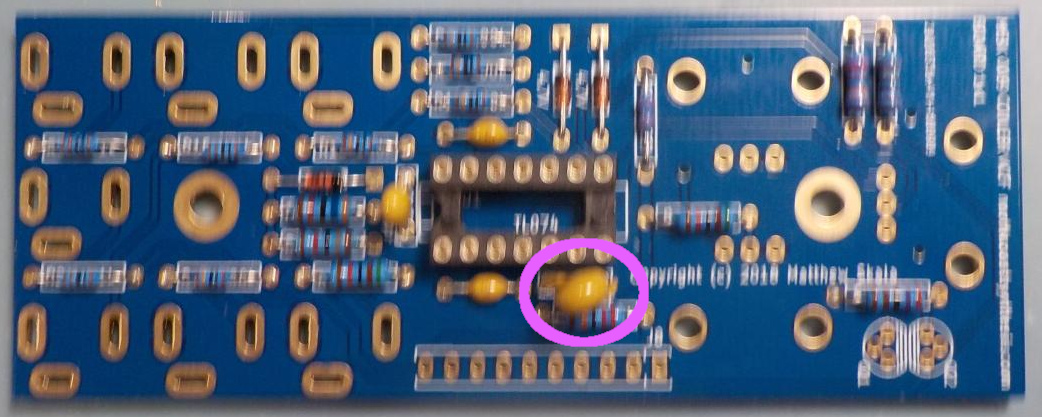
\includegraphics[width=\linewidth]{cap-100p.jpg}

\pagebreak

\section{Exponential converter cluster}

Because of the somewhat unpredictable behaviour of the coils, it is not
realistic to expect really accurate voltage-to-frequency tracking of the
Coiler VCF.  The frequency CV inputs at maximum sensitivity are called
1V/octave to give some idea of the scale of voltages users might like to
use, not as an accurate frequency standard.  However, the circuit does
contain partial temperature compensation to reduce unintended frequency
changes as the module warms up.

For the temperature compensation to work as intended, the two transistors Q1
and Q2 should be kept at the same temperature.  This is accomplished by
mounting them face to face and tightening a nylon cable tie around them to
keep them pressed together.  If you have built a North Coast Synthesis
Leapfrog Filter you will recognize the similar design; the Coiler, however,
omits the thermistor used in the Leapfrog.  Constructing this cluster of
components is a little tricky and annoying; follow the directions carefully.

\nopagebreak
\noindent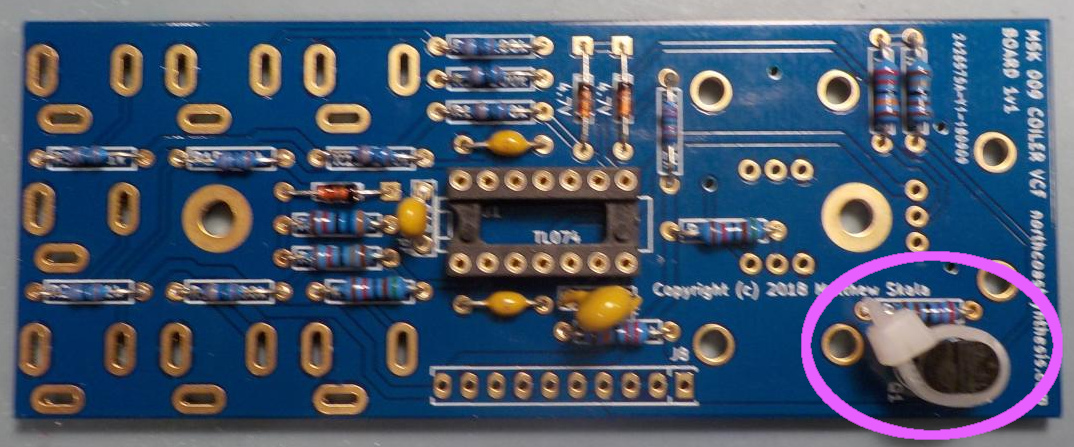
\includegraphics[width=\linewidth]{expocon1.jpg}

Insert the two SS8550D or PN200A transistors Q1 and Q2 in the board.  Do
not solder them yet.  Put a nylon cable tie around the transistors and
tighten it far enough to hold them loosely together.  Concentrate in
particular on having the two transistors meet as cleanly as possible, with
the two fully flat sides in contact.  Do not overtighten the cable tie or
cut it off yet.  This is probably the hardest step, and North Coast kits
include a spare cable tie for use in case you ruin one.  Be aware that the
components should not stick out any further above the board than is normal
for other TO-92 components; if you seat the transistors too high up, at the
full length of their legs, you may exceed the 11mm of clearance between this
board and Board~2 above it.

\pagebreak

Solder the components.  Then tighten the cable tie the rest of the way and
cut off the excess.

\nopagebreak
\noindent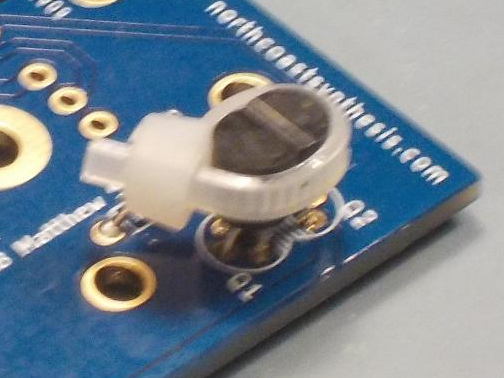
\includegraphics[width=\linewidth]{expocon2.jpg}

\section{Board to board connectors}

Fasten the two 13mm standoffs on the back of Board~1; that is the side
opposite the components already installed.  The male ends of the 13mm
standoffs should pass through the mounting holes in the board and mate with
the female ends of the 11mm standoffs on the front or component side of the
board.

Mate the 10$\times$1 header connectors J8 and P1 and place them (do not
solder yet) in the J8 footprint on Board~1 with the legs of the female
connector J8 going through the board.

Place your completed Board~2 from the previous chapter on top of the
assembly, component side up with the legs of P1 going through the P1
footprint, and fasten the board to the 11mm standoffs with the two hex nuts. 
The resulting temporary assembly should be as shown in the photo.

\nopagebreak
\noindent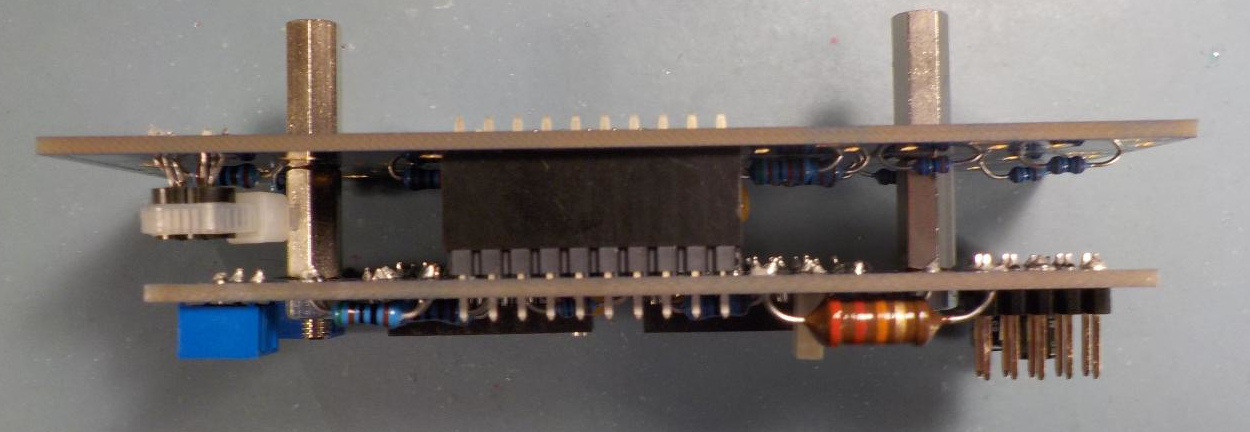
\includegraphics[width=\linewidth]{temp-assy.jpg}

Solder J8 and P1 in place on the two boards.  Then remove Board~2 and the
hex nuts holding it in place, but keep the standoffs that go through
the holes in Board~1.

\section{Panel components}

Flip Board~1 over; you will now be installing the components that go between
it and the panel.  The pieces fit together in a straightforward way, but
see the exploded assembly diagram on page~\pageref{fig:exploded} if
further clarification is needed.

Place (do not solder yet) the seven phone jack sockets J1 through J7 in
their footprints.  These are for patching signals to and from other modules. 
These components should only be able to fit into the board in one way.

\nopagebreak
\noindent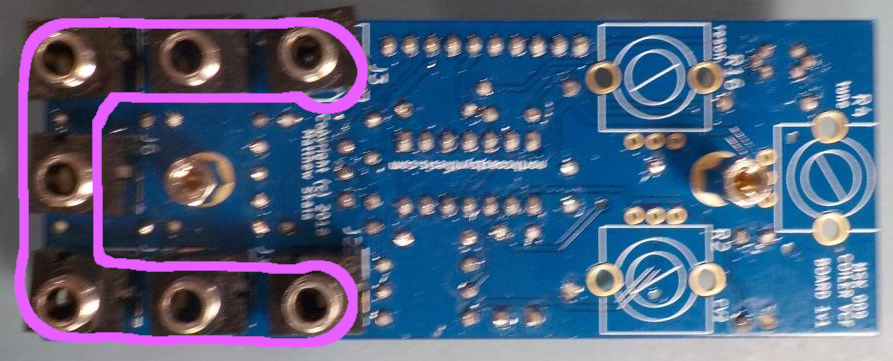
\includegraphics[width=\linewidth]{jack.jpg}

Place (do not solder yet) the three panel control potentiometers R2, R4, and
R16 in their footprints.  These are for patching signals to and from other
modules.  These components, too, should only be able to fit into the board
in one way.

\nopagebreak
\noindent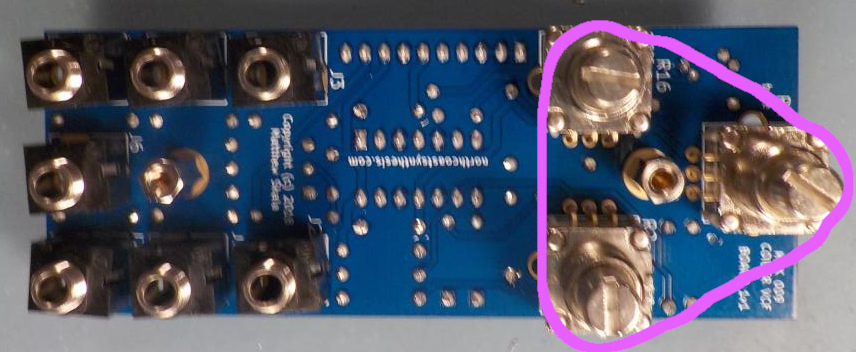
\includegraphics[width=\linewidth]{pot-100k1.jpg}

Line up the panel on top of the asembly and fasten it in place by driving
the two machine screws through their corresponding holes into the 13mm
standoffs.

\pagebreak

Install all the hardware for the panel components.
In the case of the potentiometers, the sequence is first (nearest
the panel) the conical spring washer, high side in the middle and low side
around the outside; then the toothed lock-washer; then the nut.  If the
teeth on the lock-washer seem sharper on one side, that side should be up,
facing the nut.

In the case of the jack sockets, the knurled nuts provided for these will
have screwdriver slots on one side, and those should face the outside with
the smoother side facing the panel.  You may need to tilt the assembly and
jiggle it a bit to get the jack sockets to fall into the right alignment
with their bushings poking through the panel.  On the other side, when
correctly installed their solder legs will just
barely pass through the circuit board.

Do not overtighten any of this hardware, and be careful, if you are
using wrenches or pliers, to avoid scratching the panel.  Wrapping the tool
jaws with tape may help.

\nopagebreak
\noindent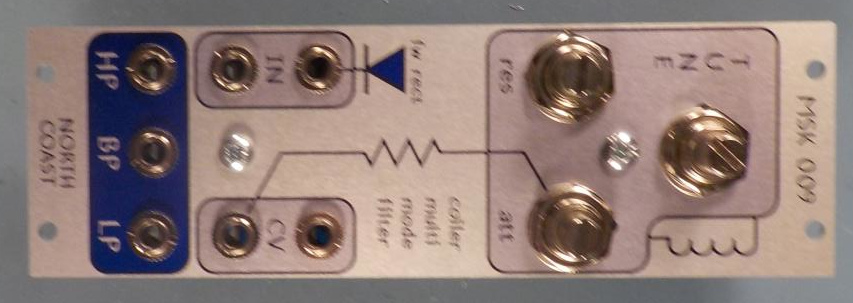
\includegraphics[width=\linewidth]{attach-panel.jpg}

\pagebreak

\section{Final assembly}

Insert the TL074 chip in its socket on Board~1.  Be careful to insert it
right way round:  the end with Pin 1 will be marked by an
indentation at one corner or a notch in the end and this end of the chip
should be inserted to match the notch in the socket and on the board
silkscreen and the rectangular Pin 1 solder pad.  The Pin 1 end of the chip
is at the bottom when the module is inserted in a rack.

Also be careful all the legs of the chip go into the corresponding
holes in the socket.  These chips, when new, usually have their legs
splayed outward a little bit to help them fit snugly
into circuit boards when used without a socket and you must gently bend the
legs inward to fit them in the sockets.  If you apply
pressure to a chip prematurely, without all the legs properly fitting into
the holes, it is easy to have the legs fold up or even break off.

It should not be necessary to remove the panel from Board~1 again.  Just
attach Board~2, carefully fitting its header
plug into the header socket on Board~1 and the male ends of the standoffs
through the corresponding holes in Board~2.  Then use the hex nuts to fasten
Board~2 in place.

Insert the TL074 and LM13700 chips in their sockets on Board~2.  Be careful
to insert them right way round, with the Pin~1 markings on the chips
matching those on the board.  The two chips are oriented in opposite
directions, with the Pin~1 marking on each chip at the end furthest from the
other chip.  As with the TL074 on Board~1, be careful all the legs are in
the holes of the socket before you press each chip down, lest you fold up
the delicate legs.

There is a rectangular white area at the top of Board~2 reserved for adding
a serial number, signature, quality control marking, or similar.  Use a
fine-tipped permanent marker to write whatever you want there.  Isopropyl
alcohol will probably dissolve marker ink, so do this step after any
board-cleaning.

Your module is complete.

\nopagebreak
\noindent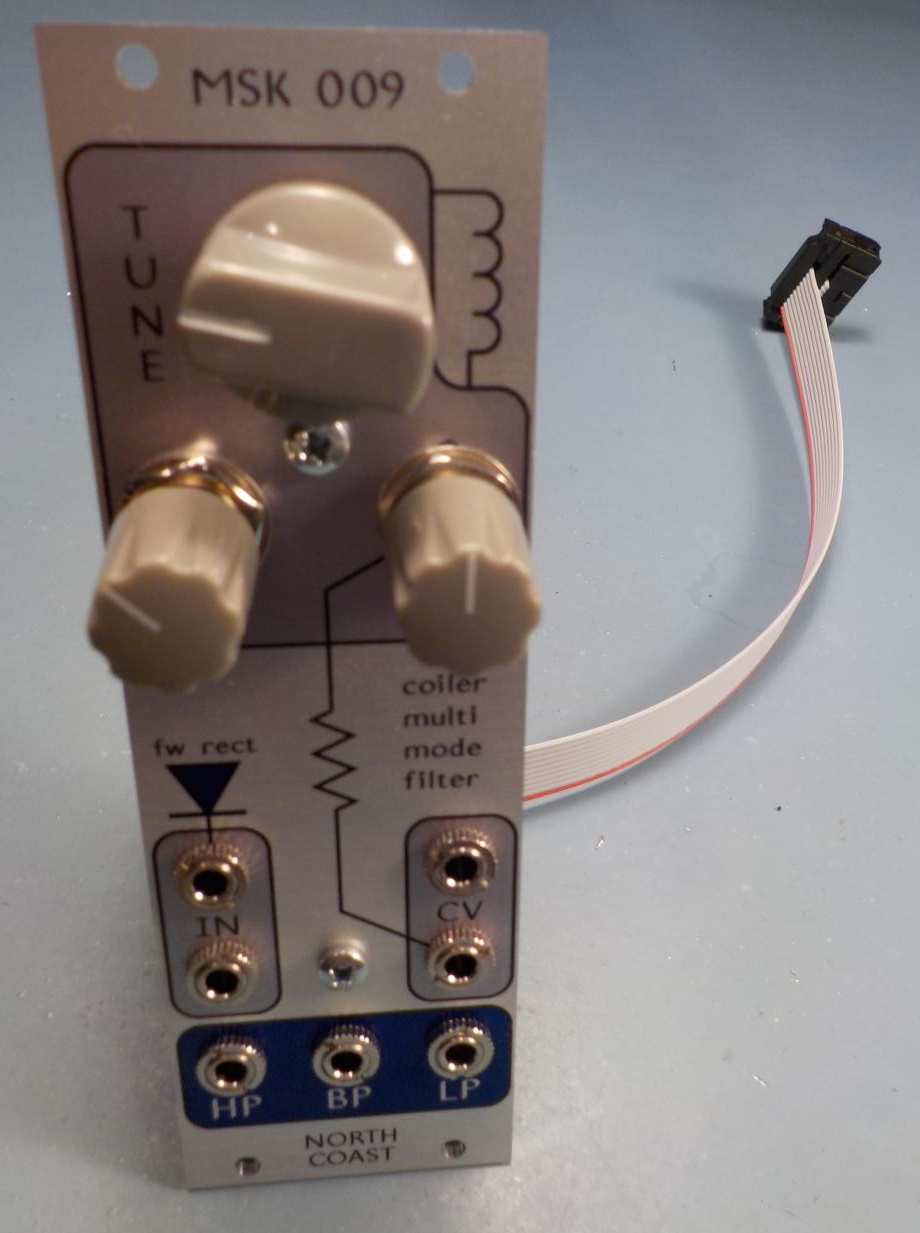
\includegraphics[width=\linewidth]{finished.jpg}
